\documentclass{article}
\usepackage{listings}
\usepackage{graphicx}

\lstset{ %
language=Java,                  % the language of the code
basicstyle=\footnotesize,       % the size of the fonts that are used for the code
numbers=left,                   % where to put the line-numbers
numberstyle=\footnotesize,      % the size of the fonts that are used for the line-numbers
stepnumber=1,                   % the step between two line-numbers. If it's 1, each line 
                                % will be numbered
numbersep=5pt,                  % how far the line-numbers are from the code
showspaces=false,               % show spaces adding particular underscores
showstringspaces=false,         % underline spaces within strings
showtabs=false,                 % show tabs within strings adding particular underscores
frame=single,                   % adds a frame around the code
tabsize=2,                      % sets default tabsize to 2 spaces
captionpos=t,                   % sets the caption-position to bottom
breaklines=true,                % sets automatic line breaking
breakatwhitespace=false,        % sets if automatic breaks should only happen at whitespace
title=\lstname,                 % show the filename of files included with \lstinputlisting;
}

\begin{document}

\setlength{\parskip}{\medskipamount}
\setlength{\parindent}{0pt}

\title{Extending SPARQL With Remote OWL Reasoning}
\author{Luke Slater (lus11@aber.ac.uk)}
\date{February 2014}

\maketitle

\pagebreak

\section{Introduction}

The nature of my project builds on technologies concerned with the semantic web.
Pioneered by Tim Berners-Lee and the W3C, the Semantic Web exists as a set of
recommendations, standards and technologies which support structured and
federated information sharing on the World Wide Web - primarily for
machine-readable purposes.

One particularly useful indication for semantic web technologies is knowledge
representation in the form of ontologies. Ontologies store information about
objects and then represent their hierarchies and interrelations using axioms.

For the practical use of these knowledge representations, both users and
programs need to be able to easily query and reason with the data to gain
meaningful results. 

Such technologies are commonly found in are the fields of biology and
medicine - which utilise and mine ontologies for the purpose of creating new
information in fields such as drug creation and repurposing, as well as the
standardisation of medical terms between institutions.

There are several types and tiers of semantic web technologies used for
knowledge representation, the most popular of which are RDF and OWL - which
provide different features for such purposes.

RDF is a graph-based technology by which data is stored and labelled about
models, while OWL generally describes the structure, relationship and and
hierarchies between objects. This kind of structured data approach means that
through datastores and ontologies we can actually represent meaning in data.

OWL ontologies exist to describe objects such as drugs, genes or biological
components, while RDF will describe the actual models or instances of these
objects. In RDF datastores, particular items are often annotated with references
to objects described in OWL ontologies using their IDs.

However, while these annotations exist there is no easy way to relate them, or
to integrate them together in a query - for example, a query to find all models
in an RDF datastore annotated with the ID of a particular object from an OWL
ontology. Currently, one must manually look up the ID of an OWL object using
desktop software such as Protege, and then implant this manually into a SPARQL
query to find associated models in RDF datastores.

Therefore, this project is concerned with interlinking RDF and OWL querying
technologies. The goal is to allow users to write simple queries for OWL
ontologies inline in a SPARQL query - which may return one or many object
identifications - and then use the results to query for data in an RDF store.

To do this, an extension will be developed for the SPARQL language in the form
of an OWL construct, which will allow the language to execute several types of a 
given OWL query at a given OWL endpoint, and then retrieve these results and use 
them in the SPARQL result-set.

The query itself will comprise of a Manchester OWL Syntax\cite{manchesterowl}
string. This is a simple OWL ontology
language developed to mirror natural language and ease the use and demonstration
of ontology constructs. While originally developed as a
language by which to define ontologies, certain applications such as
Protege have used the language in a novel manner, providing functionality to
query OWL ontologies for objects using the syntax.

To make this possible, this will also require the development of a manner by
which to easily make human-writable OWL querying possible over the Web. While 
RDF has a highly developed query language (SPARQL), OWL does not have a 
universally and easily available method for querying data over the web. 

Solving this problem will involve the creation of a simple HTTP API for reasoning 
and querying OWL ontologies, mirroring the functionality of the SPARQL Endpoint. 
It will accept a class description in the
form of a Manchester OWL Syntax string, as well as a number of options and then
apply these to a number of configurable loaded ontologies, and return the
relevant classes in a machine-readable format. 

Beyond the necessitation for development in extending SPARQL with OWL reasoning, 
the work will also provide a service in that the development of a web-based OWL 
endpoint will further the availability and accessibility of easily queriable
OWL data on the World Wide Web. This will bring further feature parity between
RDF and OWL technologies, since the endpoint will parallel a SPARQL endpoint,
and potentially open up further use for OWL technologies in a wider range of
technologies and softwares.

Furthermore, I will endeavour to create a working implementation of this
addition - which will allow a demonstration of the system. The particular 
focus of my resulting work, beyond the primary functionality
will be in creating software that is easy to maintain, extend and modify - in
the spirit of open data and the semantic web.

Achieving this will require research into the various technologies on the
semantic web (such as RDF, SPARQL and OWL) and the fields which underlie them
(such as description logic). Then, research into the various pieces of software
and applications which work with semantic web data will take place to find the
most suitable and practical solution for the development of this project.

\section{State of The Art in The Semantic Web}

The Semantic Web is a set of technologies, methodologies and standards suitable for
generalised data expression, transmission and processing over the World Wide
Web. Before the Semantic Web's philosophical beginnings in
2001, the World Wide Web had seen massive success as a platform for the
sharing of resources intended for reading and interaction by humans.

However, most of the data existed in the format of forward-facing 
documents accessible via URLs, content comprising of arbitrary natural language
along with human-intended formatting and navigation techniques. This is
sometimes referred to as the \emph{syntactic web}, describing a situation in
which data is only given meaning by off-line consensus and arbitrary agreement -
the primary relevant example being natural language.\cite{syntweb}

This approach means that the data contained on the World Wide Web at large is
generally unstructured; the downside of this is that without using advanced 
natural language processing techniques, it's very difficult to then have
software garner meaning from, and thereby process, manipulate and intercommunicate 
the data in a generalised and useful manner.

Therefore, the philosophy of the semantic web acknowledges this need for a
reconciliation of certain data in a format which software can deal with. The
original Semantic Web manifesto\cite{semweb} describes the vision of a 
futuristic world of home automation and software intercommunication serving 
the human lifestyle, backed by standardised data formats which allow software to 
easily traverse and process the totality of available data over a federation
of structured data. This forms the
underlying philosophy and school of thought for ubiquitous computer science -
whereby computing evolves from its traditional role as directly
human-interactable and controlled devices for specific purposes, to become
integrated further and more deeply into every aspect of human life 
in a latent manner.

Examples given are those of a user being able to easily find an appropriate
doctor's appointment, with the conditions that a doctor is nearby, available, 
suitable for treating a particular condition and that such an appointment would
not clash with the patient's timetable.

To achieve this, structured data would be available for gaining data on:
physical locations, doctor specialities and timetables for both the doctor and
the originator of the request. 

In the current day, it is likely that all of this information actually exists in
a digitalised manner - however such systems do not intercommunicate due to no
standard format or technology for the interpolation and processing of this data
from several sources using a standard interface. 

These ideas constitute the concept of linked data, striving to utilise the World 
Wide Web's capacity and infrastructure for intercommunication, creating a 
publishing paradigm for linked structured data\cite{linkdata} which can be
queried and used practically by software at will.

To move forward and implement the Semantic web, we have since that date seen the
production of a number of technologies and standards. Today, the
Semantic Web exists as a movement promoting standardised structured data
formats, primarily led by W3C.\cite{revisited}

There are several languages and specifications which are used in the Semantic
Web, including RDF and OWL - among several technologies used to build, integrate
and query data stored in them.

\subsection{Technologies}

\subsubsection{RDF}

One of the primary and initial technologies used to represent this machine-workable data on
the web is the Resource Description Framework (RDF)\cite{rdf}, which are a set of
specifications which describe a general methodology for conceptualising and
modelling data in a graph format, intended for solutions in which the data needs to 
be processed by software.

It forms a graph of statements representing metadata about resources on the
World Wide Web in the form of simple statements in the terms of simple
properties and property values. Each RDF statement is formed of a Subject, a
Predicate and an Object - a data format commonly referred to as a triple:

\begin{description}
    \item[Subject] The object being described.
    \item[Predicate] The definition of the property of the subject being
    defined - usually given as a URI reference or URIRef.
    \item[Object] This is the value assigned to the given
    predicate-defined property of the subject.
\end{description}

For example, in the simplest terms a statement which defines the name of the author of
this document might take the form:

\begin{lstlisting}
http://users.aber.ac.uk/lus11/dissertation has an author whose value is Luke
Slater.
\end{lstlisting}

In which the subject is \emph{http://users.aber.ac.uk/lus11/dissertation}, the
predicate is \emph{author} and the object is \emph{Luke Slater}.

Usually, URIs are used to identify objects, subjects and predicates because,
since allow them to be fully-fledged resources by using externally pre-defined and
standardised vocabularies - avoiding using multiple strings to refer to the same thing.

RDF information is commonly stored, transmitted and worked with using the
RDF/XML format, which is an expression of the graph data structures in the
eXtensible Markup Language (XML)\cite{xml} - a language designed to store and encode
documents (as opposed to HTML, which is for formatting data). 

Therefore, the example triple given above, may be stored in RDF/XML format as
follows:

\begin{lstlisting}
<?xml version="1.0"?>

<rdf:RDF
xmlns:rdf="http://www.w3.org/1999/02/22-rdf-syntax-ns#"
xmlns:eg="http://www.w3schools.com/rdf/">

<rdf:Description rdf:about="http://users.aber.ac.uk/lus11/dissertation">
  <eg:author>Luke Slater</si:author>
</rdf:Description>

</rdf:RDF> 
\end{lstlisting}

There are a number of other serialisation formats for RDF data,
including:

\begin{description}
    \item[Turtle] This is a compact and human friendly format for storing RDF
    data, providing abbreviations and short forms for common syntaxes and
    data types. Often used for examples and tutorials.\cite{turtle}
    \item[N-Triples] A simple line-based language which is not as compact as 
    Turtle, but is easier to parse and demonstrates the underlying 'triple'
    pattern of RDF (Subject, Predicate, Object).\cite{ntriples}
    \item[N-Quads] An extension on N-Triples used for the serialisation of
    several RDF graphs.
    \item[JSON-LD] A JSON based serlisation of RDF data. Universally easy to
    parse and process using client libraries in a multitude of different
    languages. Naturally suites key-value datastores very well.
    \item[N3] A specification very similar to Turtle, but allows some additional
    features such as the specification of inference rules (RDFS).
    \item[RDF/XML] The most common serialisation format, and was developed as
    the reference implementation for the RDF specification. Used to be in heavy
    use but users have recently been preferring other formats due to their
    friendliness both for users and machine-based processing - among this,
    certain RDF graphs are not able to be represented in RDF/XML due to
    restrictions on namespaces permitted by the XML syntax.
\end{description}

However, all of these actually represent a graph data structure, which is shown
for the example in figure \ref{rdfexample}.

\begin{figure}[h!]
  \centering
  \includegraphics[width=\textwidth]{rdfexample.png}
  \caption{Example of an RDF Graph}
  \label{fig:rdfexample}
\end{figure}

The Web and applications on it currently use a wide range of methods to store
and serialise and thereby process and communicate structured data. These include 
XML, JSON, YAML and various relational database systems which store binary
representations of data such as MySQL.

While XML and other data serialisation formats already exist, and allow for easy 
storage, transmission and manipulation by machines, there is an issue in that 
applications which use them often define their own schemas and constructs for 
data description. This is useful for the application itself and for applications 
which subscribe to its data schema, but requires extra work for applications which 
wish to use it. Using RDF, there is a standard data format, therefore meaning
every application knows the structure and schema used to describe a document.

While key value data stores (such as Redis or MongoDB) have many advantages over 
Relational Database Management Systems (RDBMS), RDBMS have the advantage that for 
certain datatypes,
for example a 'date' are centrally configured and understood by all instances of
that database driver (MySQL, for example). Key-value data is much more freeform,
consisting of a key and a value - and therefore there are no centrally
standardised or understood meanings for data represented.

RDF strives to solve these problems, creating a universal and general
specification for resource description, by providing a known data format with
widely known vocabularies included in predicates within the data to describe 
the datatypes within it - the existence and extensibility of said vocabularies 
meaning it can universally define and describe much more complicated, customised
and
specific datatypes than can RDBMS systems (as well as already including a number
of built-in datatypes for general use, such as xsd:int). 

Additional to RDF, the RDF Schema\cite{rdfs} technology was later developed. This is
designed to buld on the limited vocabulary of RDF to provide additional features
for knowledge representation by providing additional syntax for describing
classes. An example of this is the ability to describe a class's types or
relationships between types.

\begin{lstlisting}
PREFIX animal: <http://realispicio.us>
animal:turtle    rdfs:subClassOf    animal:animal
\end{lstlisting}

The above example shows the description of a cat as being a subclass of animal.
The addition of this kind of data representation constitutes a simple IS-A
relationship as per description logic\cite{desclogic} - and through 
doing so allows the data to actually represent meaning through the class 
interrelations and restrictions (or axioms) in an \emph{ontology}.

However, RDFS only supports the EL family of description logics and is therefore
extremely limited in terms of its expressive power - only being able to represent 
subclasses and subproperties (subsumption) between data.

\subsubsection{OWL Ontologies}

An ontology\cite{ontology} is a formal representation of a set of concepts and their
interrelationships, types and hierarchical standings. RDF (and RDFS moreso) is
rather naturally suited to storing this type of data, being that it represents 
a graph. However technologies such as OWL (The Web Ontology Language) have been 
developed post-RDF to provide additional suitability and a greater featureset 
for this paradigm of knowledge representation, instead of graphs using a 
model-based paradigm for data representation.

Previous to OWL, there has been a long history of the attempt for knowledge
representation in the field of computer science, and particularly
artificial intelligence in which ontological thinking began as a purely
theoretical field. Practical implementations grew from the initial idea of 
storing machine-readable data alongside semi-structured and forward facing HTML
documents in the semantic web movement. 

\begin{description}
    \item[SHOE] Simple HTML Ontology Extensions were developed to create simple
    extensions for the HTML language to allow semantic metadata to be included
    inline. Developed around 1996, it is considered a precursor to the larger
    semantic web movement.\cite{shoe}
    \item[OIL] The Ontology Inference Layer\cite{oil} was a previous attempt at creating
    an ontology infrastructure in the Semantic Web, and is similarly based on
    the concepts of description logic.
    \item[DAML] DAML\cite{daml} was an early attempt to provide structured relationships
    between semantic data on the web, developing a language related to XML more
    suited to describing the relationships between objects.
    \item[DAML+OIL] This project worked to combine the works of OIL and DAML, to
    create a syntax layered on RDF and XML (essentially an extension of RDFS) which 
    could be used to create ontologies describing classes and rulesets which governed 
    relationships between them.\cite{damloil}
\end{description}

These previous research projects and their resulting technologies were the
precursors to the OWL technology, and eventually their concepts formed much of
the basis for the OWL ontology framework.

Despite the misleading acronym, OWL itself actually encompasses a large amount of
different individual technologies, languages and profiles depending on the version of the 
specification used and the set of features necessary for a given exercise in knowledge
representation - as well as whether humans or machines are the primary audience 
for use. 

Initially, there are several serialisation formats and lanauges which can be
used to describe an OWL ontology:

\begin{description}
    \item[RDF/XML] A common format used to serialise ontologies, providing
    mappings for OWL constructs and can express many axioms
    reasonably. As an extension, these can also be described by the alternative
    RDF serialisation languages listed above. This means the ontologies can also
    be described in the number of RDF serialisation formats described above.
    \item[OWL2 XML Syntax] There is a particular XML format specification which
    describes the serialisation of a full OWL ontology within it.\cite{owl2xml}
    \item[Manchester OWL Syntax] A compact and human-readable syntax which can express
    either full OWL ontologies or be used (in novel cases) to describe class
    expressions for an OWL ontology. However, not all OWL constructs can be fully
    expressed using this syntax at present.\cite{manchesterowl}
    \item[Functional Syntax] Allows ontologies to be written compactly through
    methods such as provision of IRI truncation.
\end{description}

A commonly used language for the human representation of OWL ontologies both for
practical and educational purposes is Manchester OWL syntax, which can be used to 
describe full ontologies:

\begin{lstlisting}
Prefix: a: <http://realispicio.us/owl/animals/>
Ontology: <http://realispicio.us/example.owl>

ObjectProperty: eats
  Domain: Animal
  Range: Food

Class: Animal
Class: Squirrel
  SubClassOf: Animal
  EquivalentTo: eats only Nuts
Class: Turtle
  SubClassOf: Animal
  EquivalentTo: eats some People

Class Food
Class: Nuts
  SubClassOf: Food
Class: People
  SubClassOf: Food
\end{lstlisting}

The above example is the definition of a small OWL ontology with a small set of 
classes and some relationships between them. Similar to RDF it
may also contain a set of prefixes usable for shortening URIs. Each ontology
must also be identified by a unique URI, stated in the Ontology declaration.

Ontologies include a set of classes, which describe objects within the appropriate 
domain (much like a declarative RDF description of an object with a set of predicates 
and values). It also contains a set of axioms, or constraints, which describe the 
interrelationships between the classes and in essence assign meaning to the
data represented in the ontology.

Ontologies can also include instantiations of classes, much like the
instantiation of a class in object orientated programming languages.
Similarly, it must include definitions for each of the properties, which 
must abide the axioms described by the class definitions.

The set of available axioms, constraints and relationships available in OWL
ontologies allow it to effectively model description logic\cite{desclogic}. 

The mainstay object relation found in knowledge representation and description
logic is that of IS-A; a relationship whereby one class is a subclass or 'type'
of another - the definition of the superclass then implying that of the
subclass. This is achieved in OWL ontologies with the 'SubClassOf' axiom,
evidenced above by describing that the Squirrel and the Turtle are both
subclasses of Animal, while Nuts and People are subclasses of Food.

Another common axiom described in ontologies are existential quantifications, or
rather, expressing constraints on a property assigned to a class. Above, we
define the object property 'eats' to all animals, noting that it can contain any
type of food. Furthermore, we then set additional constraints in the definitions
of each animal - squirrels can only eat nuts, while turtles must eat some
people.

There are various classes or 'families' of description logics which provide various 
types of rulesets and axioms at varying levels of complexity; following are some basic 
families found in the realm of knowledge representation:

\begin{description}
    \item[EL] A small description logic which provides conjunction (AND) and
    existential quantification - supported by RDFS.\cite{rdfs}
    \item[EL++] The most common description logic used in ontologies - an
    extension of EL logic designed to be minimal while containing the main 
    expressions used by large-scale ontologies for most practical 
    applications.\cite{elplusplus}
    \item[SHIQ(D)] Popular description logic for ontologies and reasoners which
    supports role hierarchies, extra cardinality restrictions and other
    features.\cite{shiq}
\end{description}

Both of the axioms used in the animal ontology described above would be
supported by an RDFS ontology, since it supports the EL family of description
logics (IS-A and existential quantification) - however more advanced axioms
included in other description logics require more expressive power - provided by
OWL ontologies.

Despite being a simple ontology, the logical implications of even a small set of
axioms are great (though not necessarily explicitly stated, especially in the
case of existential quantification). For example, an individual turtle as described 
above would be considered to pass the rules of the ontology only if they eat some 
people, therefore a turtle is free to eat nuts. On the other hand, a squirrel is limited
to eating only nuts - so a squirrel observed eating people is likely not a squirrel at all.

The testing of implications of the description logic used to represent
knowledge in OWL ontologies is supported by semantic reasoners, which are 
pieces of software designed to evaluate the set of axioms between classes for 
logical consistency. OWL succeeds many previous attempts at ontological 
representation due to the existence of complete and terminating reasoners 
which can fully evaluate every consequence of the logic which exists in an 
ontology, allowing larger and more complicated ontologies to exist while 
continuing to contain validated consistent meaning.

There are several OWL variations, which exist as variants of the full OWL
specification and differ depending on their expressive power.

\begin{description}
    \item[OWL LITE] Designed to support cases in which ontologies require only
    the definition of classes and their basic hierarchies, also supporting
    limited cardinality constraints. Originally developed as a first-step
    migration choice for ontologies currently implemented in other systems. Not
    in wide use, since constraints can easily be broken with complicated rules
    amounting to similar implementation complexities found in OWL DL.
    \item[OWL DL] A sublanguage designed to provide maximum expressive power,
    while retaining terminability and decidability. It includes all OWL language
    constructs, though places certain restrictions upon cases in which they may
    be used. 
    \item[OWL Full] Uses different semantics to the other OWL sublanguages, and
    is designed with compatibility with RDFS in mind. This means it is
    undecidable, and therefore standard OWL reasoning software cannot be
    performed on such ontologies.
\end{description}

There are also OWL profiles\cite{owlprofiles}, which are variations on the OWL
language specification, which trade some features for the efficiency of reasoning.
Each implements different sets of description logic families, tuned to differing
knowledge representation approaches meaning each is useful in different situations.

\begin{description}
    \item[OWL 2 EL] Designed for very large ontologies which include many
    properties or classes. The profile is based on the EL++ family of 
    description logics, which include existential quantification. Therefore,
    basic reasoning can take place in polynomial time in relation to the size of
    the ontology.
    \item[OWL 2 QL] For applications which include large amount of instance data
    (instances of classes, tantamount to records in a relational database), The
    expressive power of this profile is very limited, though includes most basic
    modelling concepts. Answering queries with this profile can be done with a
    standard relational query (such as SQL).
    \item[OWL 2 RL] Useful for situations in which scalable reasoning is
    required, while simultaneously not being able to sacrifice much expressive
    power in the ontologies.
\end{description}

Different semantic reasoners have different featuresets - generally
implementations of reasoning for various axioms found in ontologies, or
completeness of various reasoning methods. These are generally to curtail 
the time and resources needed to reason with large ontologies. The various
reasoners generally aim to support all features contained within a specific OWL
profile\cite{reasonercompare}\cite{reasonerbenchmark}.

\begin{description}
    \item[Sesame] Open source software for reasoning with with RDF and RDFS
    information\cite{sesame} - deals with OWL ontologies only on the level of RDF graphs.
    Allows connections to various RDBMS, including MySQL and PostgreSQL.
    \item[OWLIM] Uses the TRREE engine for RDFS and OWL reasoning. Offers
    configurable reasoning support and performance for various uses. By default,
    it performs reasoning and query evaluation in memory.\cite{owlim}
    \item[KAON2] A Java reasoner which implements an extension of SHIQ rules with
    extensions for DL-safe rules (a certain subset of axioms and rules which
    ensure decidability).\cite{kaon} It utilises novel methods to apply known
    deductive techniques such as magic sets or join-order optimisations
    to DL reasoning, making it particularly useful for reasoning over ontologies
    with large ABoxes.\cite{kaonabox}
    \item[HermiT] Fully supports DL rules, though support for full SHIQ is still
    in progress. The algorithms used are much more deterministic than others in
    use.\cite{hermit}
    \item[RacerPro] Optimised tableau reasoner for SHIQ(D). Supports integers
    and real numbers. Implemented in LISP and is commercial
    software.\cite{racerpro}
    \item[Pellet] Supports SROIQ reasoning with simple data types, supporting a
    tableau based decision procedure.\cite{pellet}
    \item[ELK] Ontology reasoner with the primary goal of supporting the full
    OWL 2 EL profile in a fast manner. Still somewhat in progress, but is included
    in OWLAPI as a default reasoner.\cite{elk}
    \item[FaCT++] Reasoner which implements the tableau procedure to support the
    OWL DL language, including further data types such as strings and
    integers.\cite{fact}
\end{description}

The approaches a reasoner takes to confirm satisfiability and consistency of
a knowledge base differ, but generally begin with normalisation and then
conversion to an internal format. 

The knowlege base is generally seperated into seperate 'boxes' used for
reasoning. The set of axioms applied to classes in the ontology are seperated
into what is commonly referred to as the \emph{TBox}, and then a set of axioms
which apply to class instances are seperated into the \emph{ABox}. 

Following this, reasoners compute and cache the taxonomy of the ontology before 
finally performing a satisfiability check.

Many reasoners (e.g. Pellet and RacerPro) use the analytic
tableau\cite{tableau} method for
reasoning, which determines the satisfiability of sets of rules or formulas
representing first-order logic; the aim being to progressively simplify formulae
until rules are exhausted or maximum simplicity is reached, deciding subsumption
problems for pairs of concepts in the ontology.

Other reasoners, such as KAON2, use algorithms which convert the knowledge base 
to a Disjunctive Datalog Program.\cite{ddp}

\subsubsection{SPARQL}

Previously, languages used for the representation of various types of ontologies
were described, these are designed to be interacted with by machines - however,
a number of technologies also exist for human-interaction with the datastores
including querying and data manipulation.

SPARQL\cite{sparql} (SPARQL Protocol And RDF Query Language) is a query language similar to
SQL which allows the querying and manipulation of RDF (and similar) datastores.
This is a human-interactable language, which means that while it has a
non-freeform syntax it is designed to be used by humans (as well as computers)
to interact with data on the semantic web.

SPARQL queries usually consist of the following\cite{sparqlquerying}:

\begin{description}
    \item[PREFIX] A list of prefix declarations, which can be used to shorten
    and simplify URIs in the remainder of the query.
    \item[FROM] Describes the dataset to query, usually a URI pointing at an RDF
    dataset.
    \item[SELECT] Describes the data to include in the resultset.
    \item[WHERE] Describes the data to query for in the dataset.
    \item[MODIFIERS] These allow you to apply modifiers to the resultset, such
    as a limitation on the total results or a pattern for ordering.
\end{description}

Less commonly there are also CONSTRUCT, which allows you to pull full triples of
data from a store.

SPARQL also has the provision to query data from non-RDF databases such as Redis
and OWL ontologies by transforming and interacting with the data as if it were
in an RDF syntax. This is useful for data integration, as it means data can be
used over multiple formats. However, certain OWL representations cannot be
converted by most RDF readers - including functional syntax, Manchester syntax
and OWL/XML, and in converting an OWL ontology to RDF format, richer semantics
offered by OWL are lost - including certain axioms, and on-the-fly reasoning.

Another important quality of SPARQL is that it's federated, data may be loaded
remotely over the web by providing an IRI to the datastore. Also, the language
includes a 'SERVICE' keyword, which allows a query to be sent to a remote SPARQL
endpoint and be executed and results be returned and included in the
resultset.\cite{sservice}

A SPARQL endpoint is a simple interface which accepts a HTTP query including a
query parameter, then runs the query and will return the results in one of 
several machine-readable formats (usually JSON or XML). This means a wide array
of applications can easily make use of the data SPARQL deals in - one example
being Virtuoso. It also means that simple online interfaces can be developed for 
working with SPARQL. These qualities mean that SPARQL makes RDF very universally
available for use.

\subsubsection{Manchester OWL Syntax}

Manchester OWL Syntax is a class of OWL language which is designed to be compact
and human-friendly, primarily developed to provide a near human-language syntax
for interacting with ontologies for use by non-logicians who work in scientific
domains which make use of ontologies - thereby making it easier to work with in
a wider range of domains.\cite{manchesterowl} It can be utilised to represent full OWL
ontologies, however its method of using a frame based approach to data
representation means that certain ontologies cannot be directly analogoous to
other forms of ontology serialisations - however simple transformations can be
applied to extract axioms from frames and thereby represent the same ontology in
a more traditional format. 

Beyond the syntax's primary uses as a simple syntax for the explanation of
ontologies in a human-readable format, certain applications such as Protege
utilise the language to allow users to provide a simple set of criteria as a 
Manchester OWL Syntax string. These are then converted to a format which
constitutes a class description and can be used to return a set of relevant
classes within an ontology which fit the query. 

To support this, such applications apply further extensions to the language
which allow a more human-friendly to the syntax by allowing the natural IRI
identifier for a class to be replaced with a human-readable string - using the
label string included in the class definition such as \emph{fish}, rather than
its IRI such as \emph{GO:3218742}.

With such extensions, one could make a query of the example ontology described
above with such a string:

\begin{lstlisting}
Animal that eats some Human
\end{lstlisting}

The above example represents a class description which begins with a class
\emph{Animal}, describing that all matches in the expression must be subclasses
of Animal. It goes on to use \emph{that eats} to replace a restriction on the
\emph{eats} property of an animal, then defining \emph{some Human} - meaning the
property eats must contain the Human class.

This is relatively close to how this description may be described in a natural
language sentence: \emph{An animal that eats humans} (the ommision of 'some'
possible in the English language since it is inferred by the lack of a
restriction such as 'only').

Several other features of Manchester OWL Syntax also make it particularly
suitable for querying classes, compact keywords for the existential quantification 
of class properties are automatically formed as a part of the syntax after
inferences are computed. For example, if a \emph{Person} object had a 'name'
property, one could use the \emph{hasName} keyword.

However, these uses are considered novel, and are not directly supported by the W3C
specification for Manchester OWL Syntax which describes the language purely as
one for the full representation of an ontology. As such, these uses are relatively rarely
implemented, and while they are available in certain desktop applications there
exists no way for such queries to be made over the web.

\subsection{Frameworks and Implementations} 

\subsubsection{Jena}

Jena\cite{jena} is a large semantic web framework for Java, which provides an API for
reading several technologies including RDF and OWL, and its main uses are
the extraction of data from various database systems and re-representing them in
an RDF format. It includes ARQ\cite{arq}, which is an implementation of the SPARQL query language
alongside its own implementation of RDF model representation.\cite{jenardf}

However, while Jena is a large and well supported application, it suffers 
from a lack of extensibility, evidenced by a very large and widely undocumented 
codebase. This means that it's rather difficult to use its implementation of
SPARQL for additions or modifications to the syntax.

\subsubsection{OWLAPI}

OWLAPI is a Java library framework for manipulating OWL ontologies for a number of
purposes, and is the reference implementation for the OWL standard from W3C. 
It also allows users to load, manipulate and reason with OWL ontologies and has 
support for several manners of OWL languages and syntaxes, converting these to 
normative OWL class expressions. It also supports reasoning ontologies with all
of the major semantic reasoners (FaCT++, HermiT, Pellet etc).

It allows users to load a number of ontologies from a number of sources, either
locally or from a given URI, then providing reasoning services and from that
point allowing the actual modification of an ontology including the addition of
axioms and then checking that logical consistency is maintained.

It also supports serialisation of ontologies in a number of different manners,
including coversion to different machine-readable storage formats, as well as
output into human readable formats including HTML (similar to generating a HTML
site detailing JavaDoc for a piece of software).

The functionality for loading several ontologies at once into one manager from
several sources means that it is a useful tool for data integration - dealing
with data from multiple sources.

For this reason, it underlies many front-facing technologies which work with OWL
ontologies, including Protege, OWLLink and Jena's OWL components.

There are alternatives for client libraries involved in manipulating OWL
ontologies, many individual reasoners include their own libraries - however the
advantage of OWLAPI is such that it supports all of the reasoners, improving
the level of universal application and reduction in work for extension in
functionality; such libraries also do not support the full set of OWL languages,
including Manchester OWL Syntax which is a human-interactable language for
querying and representing OWL ontologies.

\subsubsection{Protégé}

Protégé is an open source project which provides a desktop-based graphical user
interface for editing, visualising, building and reasoning with ontologies, which supports
the development of plugins.\cite{prot} It is considered the premier tool for working with
OWL ontologies within the scientific community.

It supports a wide range of serialisation formats, including RDF/XML, OWL/XML,
OWL Functional Syntax, Turtle, KRSS and OBO.\cite{protowl}

One of its interesting features is that of a novel use of Manchester OWL Syntax
to query classes and return those relevant (described above).

\subsubsection{OWLLink and OWLLink API}

OWLLink is a specification which defines a machine-usable API for OWL reasoners,
the reference implementation for which is OWLLink API. The OWLLink API provides
client applications using OWLAPI to access remote reasoners through providing a
server adapter to an OWLAPI-abstracted reasoner.\cite{owllink} 

The disadvantage of this software is that it requires the client application
to use OWLAPI, or otherwise requires a complicated XML structure for the
request of data - a normalised expression of an OWL class expression. This
represents somewhat of a lock-in for the client software. 

Additionally, it does not accept Manchester OWL Syntax for queries - this could 
be remedied by parsing Manchester OWL Syntax into a class description understood 
by an OWLLink server on the clientside (a provision made available by OWLAPI).

This means that what could be a relatively simple query for retrieving a number
of relevant classes given a simple Manchester OWL Syntax query must be a rather
complicated and lengthly request. While such requests are usually made in XML,
they may also take the form of functional or S-Expression syntax, which
are similarly verbose.\cite{owllinkprotocol}

\begin{lstlisting}
<RequestMessage xsi:schemaLocation="http://www.owllink.org/owllink# http://www.owllink.org/owllink-20091116.xsd">
  <CreateKB kb="http://www.owllink.org/ont/families">
    <Prefix name="families" fullIRI="http://example.com/owl/families/"/>
    <Prefix name="otherOnt" fullIRI="http://example.org/otherOntologies/families/"/>
  </CreateKB>
  <LoadOntologies kb="http://www.owllink.org/ont/families">
    <OntologyIRI IRI="http://www.owllink.org/ontologies/primer.owl"/>
  </LoadOntologies>
  <IsClassSatisfiable kb="http://www.owllink.org/ont/families">
    <owl:Class abbreviatedIRI="families:Man"/>
  </IsClassSatisfiable>
  <GetDisjointClasses kb="http://www.owllink.org/ont/families">
    <owl:Class abbreviatedIRI="families:Father"/>
  </GetDisjointClasses>
  <GetSubClasses kb="http://www.owllink.org/ont/families" direct="true">
    <owl:Class abbreviatedIRI="families:Parent"/>
  </GetSubClasses>
  <GetSuperClasses kb="http://www.owllink.org/ont/families" direct="true">
    <owl:Class abbreviatedIRI="families:Grandfather"/>
  </GetSuperClasses>
  <GetSubClasses kb="http://www.owllink.org/ont/families" direct="false">
    <owl:Class abbreviatedIRI="owl:Nothing"/>
    </GetSubClasses>
  <ReleaseKB kb="http://www.owllink.org/ont/families"/>
</RequestMessage>
\end{lstlisting}

The above request is a sample class query for an OWLLink request, which requests
classes which are:

\begin{itemize}
    \item Equivalent to Man
    \item Not a Father
    \item Are a subclass of Parent
    \item Superclasses of Grandfrather
\end{itemize}

This could be expressed in Manchester OWL Syntax as follows:

\begin{lstlisting}
Man and DisjointWith Father and SubClassOf Parent and SuperClassOf Grandfather
\end{lstlisting}

TODO: revise

Alternatively, a wrapper around the OWLLink server could be made, using OWLAPI
to convert the Manchester OWL Syntax to the class expression, then passing it to
the OWLLink server. However, this is rather inefficient as it would require an
extra external HTTP endpoint. The approach of creating a new piece of software 
based on OWLAPI with a simple HTTP server would be, in effect, cutting out the 
middleman.

\subsection{Uses and Impact}

\subsubsection{General Use}

Despite the development of a great number of standards, technologies and pieces
of software since the inception of the Semantic Web, the original
dream and plan for evolution of the wide Semantic Web remains largely unrealised
for general application.\cite{semweb}

Despite the lack of adoption of semantic web technologies for general use, there
are a few initiatives which work to make large amounts of structured data
available. The Linking Open Data project is a community driven effort to develop
a set of standards for best practice in creating large sources for linked data
on the Web, or 'data gardens'.

A good example of a 'data garden' is DBPedia, which aims to extract
information from the online encyclopaedia website Wikipedia and provide it in a
structured and machine-processable format (RDF(S)), available for free on the 
web.\cite{dbpedia} At the time of writing, it had collected information on more than four 
million objects and had collected more than 470 million 'facts' overall,
describing more than 2.6 million entities.\cite{dbpediastats}

An important thing to note about this dataset is the grand effort which is made
to make the information freely and easily available in a number of manners and
using a number of different technologies. There is a SPARQL endpoint available
for querying, along with full database downloads and a simple endpoint for
retriving information about particular subjects in a number of formats (JSON,
XML, N-Triples etc).

The underlying technology's ability to provide simple data access over the Web
means that DBPedia can be and is already used for a number of practical
applications.\cite{dbpedia-uses}

\subsubsection{Bio-informatics and Medical Uses}

However, outside the strict prediction for the technologies developed to provide
structured data for the world wide web at large, they have been used to great
effect in specific domains - primarily in biology.

An example of a common use for OWL ontologies is that of describing animal or
plant models using the descriptive logic axioms provided by OWL. The Phenotype
And Trait Ontology (PATO) has been developed as a framework which allows the
description and integration of quantitative and qualitative phenotype
information accross different levels of granularity, domains and
species\cite{pato}; rather acommunity standard for phenotype description as
used by several international consortia (e.g. Phenoscape\cite{phenoscape},
VPH\cite{vph}, IMPC\cite{impc}).

A collection of biological ontologies can be found at
OboFoundry\cite{obofoundry}, and examples of major model organism databases
include Zfin\cite{zfin}, Flybase\cite{flybase} and Wormbase\cite{wormbase}. In working with
these ontologies the previously described Protege application is primarily used. 

These are being used for example to examine biological and drug data for medical
purposes\cite{humontology}. One particular realm of interest is drug discovery,
mining existing information on the semantic web to predict the results of drugs,
and eventually predicting and finding new targets and indications for existing
drugs\cite{semwebdiscovery}.

Efforts are also being made in the medical industry to utilise the semantic web
for improved data interlinking. Several ontologies of medical vocabularies actually
already exist in various formats such as SNOMED\cite{snomed2} - however these suffer from not
being able to interlink and integrate with other data sources. Therefore, work
is going into creating RDF/OWL mappings for these
ontologies.\cite{snomed1} 

The PHARMASurveyor software has also been developed to consider a large number
of criterion to suggest a safest drug treatment regiment for a particular
patient - providing an optimised profile for treatment.\cite{psurveyor} 

\subsubsection{Commercial Use}

Semantic web technologies are also starting to see real-world commercial use.
For example, the EPIM Reporting Hub was developed as a collaborative effort
between several companies, and is primarily used by oil companies (such as BP,
ExxonMobil and MarathonOil). It gathers and integrates data into an RDF enterprise 
database and then uses semantic web querying methods to build reports on business 
intelligence, research and performance - such as daily drilling or production
reports.

Various other companies such as BBC, Facebook and Tesco also publish RDF data
online. In the case of the BBC, this is done to aid cross-site navigation by
querying for sites which may be related to a site the user is currently browsing
- for example, finding other websites for television shows in which the cast for
a show the user is currently browsing have also
starred.\cite{bbcone}\cite{bbctwo}

\section{Problem Statement}

\subsection{Statement}

\emph{The issue we strive to solve is that of creating a simple solution for querying
OWL ontologies over the web, including the SPARQL query language.}

An issue with the practical usability of OWL ontologies as a technology for the
representation of knowledge on the semantic web, is that there is currently no
way to easily query data from it in a human interactable way over the Web.
Furthermore, this issue means it is difficult to integrate data from OWL
ontologies with that from RDF datasets. 

\subsection{Justification}

\subsubsection{OWL Queries}

As described in the State of The Semantic Web, there are two categories of
languages used to represent and interact with the data: human-interactable and
machine-interactable. These generally exist as the data storage formats (such as
RDF/XML or OWL/Functional) and the query languages (such as SPARQL) which can be 
used by humans to manipulate and integrate the datastores.

For both RDF and OWL datastores it is currently easy to interact with the data
over the web in a machine-processable manner - primarily through codebases and
libraries utilising XML parsers or through bespoke libraries and server software 
such as OWLAPI and OWLLink.

For human-querying, the area is highly-developed for RDF and similar datastores, 
with SPARQL allowing users to write queries to manipulate data both locally and
through web-based endpoints. The language also supports federation through the
SERVICE keyword, which allows the user to send further data queries to remote
SPARQL endpoints and thereby further datasets.\cite{sservice} This is incredible useful for
making useful data easily available and integratable to those working with it.

However, for OWL ontologies the situation is somewhat different, the 'querying'
of an ontology at all being somewhat of a novel concept - using Manchester OWL
Syntax for such queries, a purpose for which it was not intentionally designed.

Therefore the implementation of this functionality is not ubiquitous - only a
few pieces of software carrying it. One is Protege, which is a highly popular
desktop tool for interacting, building, integrating and editing OWL ontologies;
including a query tool allowing users to return relevant classes from a given
Manchester OWL Syntax string. 

However, the limitation of Protege is that it is strictly a desktop application
- missing the functionality found in SPARQL for reasoning over the web in a
federated manner. This limits the scope of data availability, integration and
ease of use for real world application. 

On the other hand, the OWLLink server exists for querying OWL ontologies. It
sits above OWLAPI and connects to a reasoner to expose various reasoner
functionality over the web - including querying for classes. However, the API it
exposes it very complicated and does not support querying with the Manchester
OWL Syntax. This generally
both locks client applications into using OWLAPI (and therefore Java) to make r
equests, and does not allow for easy human-interactable querying. 

\subsubsection{RDF and OWL Integration}

Data integration is an important concept in the semantic web. Generally, an
ontology described a particular \emph{domain}, or set of things which exist for
a particular subject matter. Once this data has been collected and exists in a
structured format and has meaning applied to it using description logic, one can
generally combine and integrate various information from different domains to
essentially discover or 'create' new knowledge.

To do this, data integration must take place. Languages like SPARQL allow the
interpolation of data from ontologies from different sources and different
domains, manipulating them to create meaningful products. 

However, as described in the state of the semantic web there are several manners
of storing structured data on the web - differing in language, syntax and ethos
depending on history, necessary featuresets, use cases and fitness for purpose.

Indeed, it often remains necessary to integrate data from these different
sources. The multitudes of structured data found on the semantic web exist in different
formats and with different tools used to query and manipulate them.

Therefore, to garner useful information from the integration of these datasets
one must be careful to do so without compromising the features available from a
particular ontological technology.

As explained in the previous section - SPARQL is a flexible technology and allows 
data to be pulled from several different types of datastores (including Redis or an 
OWL ontology) through providing an IRI to a resource; then converting it to an RDF 
expressed datastore, and allowing regular SPARQL querying in this
way.\cite{sparqlandowl}

This makes SPARQL a powerful tool for data integration, providing a common
language usable for querying over multiple types of datasets in a single query.

However, in the case of OWL ontologies, the current process of converting the
ontology to an RDF dataset carries a number of issues and reduced
functionalities when compared to working with OWL natively:

\begin{itemize}
  \item Inability to perform on-the-fly semantic reasoning on ontologies.
  \item No ability to query the data in a native manner (using Manchester OWL Syntax).
  \item Loss of certain expressive power and descriptive logic modelling axioms available in OWL
  ontologies when expressed in RDF.
  \item Many OWL serialisation formats not supported by many RDF readers used by
  SPARQL.
\end{itemize}

Furthermore, many RDF datasets actually refer to OWL classes through
annotations, but do not actually include the classes.

Therefore, through converting an OWL ontology to an RDF-expressed datastore for
the purpose of querying with SPARQL - it compromises the endemic qualities for
which OWL is actually used.

Successful and optimal data integration between RDF and OWL datasets would allow
for querying and interpolation of the data without having to sacrifice any of
the expressive power native to either technology.

\subsubsection{Importance and Impact}

\subsubsubsection{Drug Repurposing}

As previously mentioned, one particular real of interest in the field of
Bioinformatics in relation to the semantic web is that of drug discovery -
particularly drug repurposing\cite{pharmgkb}.

Repurposing existing drugs for new applications can dramatically reduce both
the cost of drug development and the rate of attrition in new compound
development. Such a project exploits the exploration of model organism
phenotypes for the discovery of novel drug action. More specifically, it would
exploit the phenotypic similarities between classical 'loss of function'
mutations and the inhibition of protein functions by drugs.

Through doing this, one may potentially discover novel drug actions and
indications - thereby carrying a further potential to eventually find new treatments for
currently untreatable conditions. Initial studies and research have shown this
to be a faesible subject for research with potentially useful
results.\cite{drugrepurposeinitial}

It would be achieved by first integrating drug effect and model organism
phenotype data from publicly available class ontologies - utilising axioms to
integrate and compare data existing in different domains. This would be achieved
through various currently existing and  newly developed data integration techniques 
(including the SPARQL integration of OWL and RDF data), along with methods of
semantic similarity - using the layers of abstraction provided by ontologies
to compare data. Then, any similarities between drug effects and organism
phenotypes would be established. Once these are identified, one would determine 
whether the observed similarities can provide insights into drug-target relationships, 
confirming resultant hypotheses independently on human subjects through tests.
(?)

The specific advantage of this project is the ability to retrieve IDs from
OWL ontology class descriptions (such as a the id for a class for the
acetylcholine-gated channel complex - GO\_0044459) from an OWL query using a
Manchester OWL Syntax query, and then use these results to search RDF
datastores for models which are annoted using the IDs for these properties.

This is currently not possible without a user manually using a piece of software
such as Protege to manually query OWL ontologies for annotation IDs, and then
copying them into a SPARQL query to find annotated models.

\subsubsubsection{Accessibility}

One thing that seems lacking in implementations of semantic web technologies as
they exist is that the major implementations are all rather large and opaque
Java libraries - this being a language which generally requires a lot of
boilerplate - additionally, transmission formats are commonly XML, which also
requires extra overhead in processing when compared to abstract key-value
storage formats such as JSON. 

Conversely, underlying technologies and applications on the web have meanwhile 
been moving towards use of lightweight frameworks and languages. Modern applications 
have been opting for abstract key-value stores such as Redis, which suffer from
a lack of additional features available from ontologies. 

Transmission of data on the web tends to favour simple REST APIs which feature 
simple HTTP requests with parameters\cite{rest}, instead of the complicated XML structures 
necessary to query data from OWLLink servers for example. On the other hand, the
previously discussed SPARQL data endpoints provide a simple HTTP interface for
SPARQL queries, so while the underlying technology can be anything - the
interface means that any application can easily make use of the service.

The effectiveness of the availability of these simpler, more responsible and 
accessible 
technologies\cite{uptake} can be seen in the massive number of web and desktop applications
which make use of these standard interfaces and RESTful APIs. 

Therefore, I believe it may be that the lack of takeup of knowledge-representation systems
for front-end applications may be the down to the lack of lightweight libraries, 
services and frameworks available for working with them. The solution of this
problem - particularly for OWL, which provides advanced knowledge representation
features and techniques - may potentially bring about some more interesting and
practical uses for the technology; hopefully moving towards the original vision
of the Semantic Web as a universally federated and easily traversable datastore
for all purposes.

\section{Design and Implementation}

My solution to the given problems are to develop an extension to the SPARQL
query language - a block which allows a user to send a Manchester OWL Syntax query to a
remote OWL reasoner endpoint which has pre-computed inferences and upon querying
returns a set of results relevant to the class description described by the
query. These classes are then included in the SPARQL resultset. This requires 
both development of the language extension and the queriable OWL endpoint.

Being a research project whose technical output is primarily a prototypal proof
of concept, the software development methodology used was prototypal and
iterative. After researching the technologies and current software involved in
the realm of the semantic web, practical research and prototyping was done with 
several solutions - including the use of Jena and OWLLink - before settling on
the following design and implementation approach as being the most likely to
give practical results given the project's timeframe.

In terms of iteration, the requirements for a potential user were first analysed 
as per the problem statements:

\begin{itemize}
    \item Provide a simple REST-like API for users to make HTTP queries for
    classes over several reasoned OWL ontologies using a class description
    provided in Manchester OWL Syntax.
    \item Allow the user to choose to make a query for subclasses, equivalent
    classes or superclasses over OWL ontologies.
    \item Allow a user to make remote OWL class queries to a remote endpoint from 
    within the SPARQL query language.
    \item Provide a Web interface for users to make SPARQL queries with the OWL
    block extensions.
    \item Allow such returned data to be used to find RDF datastore models in 
    SPARQL annotated with the class IDs returned from OWL classes.
\end{itemize}

Thus, initially research was completed into the semantic web technologies
themselves (RDF/OWL), and then the fields which underlie them (description
logic). It was decided that SPARQL already exists as a powerful and flexible
tool for querying RDF (and similar datasets) on the web, while no such provision
existed for OWL ontologies. Therefore, it was decided that the most efficient
and practically useful approach to providing web-based OWL ontology querying was
to combine SPARQL with the compact and human-readable querying methods available
in the Manchester OWL Syntax. 

The following two pieces of software were developed to fit these requirements,
and the basic workflow is shown in figure \ref{fig:sparqowl_request}.

\begin{figure}[h!]
  \centering
  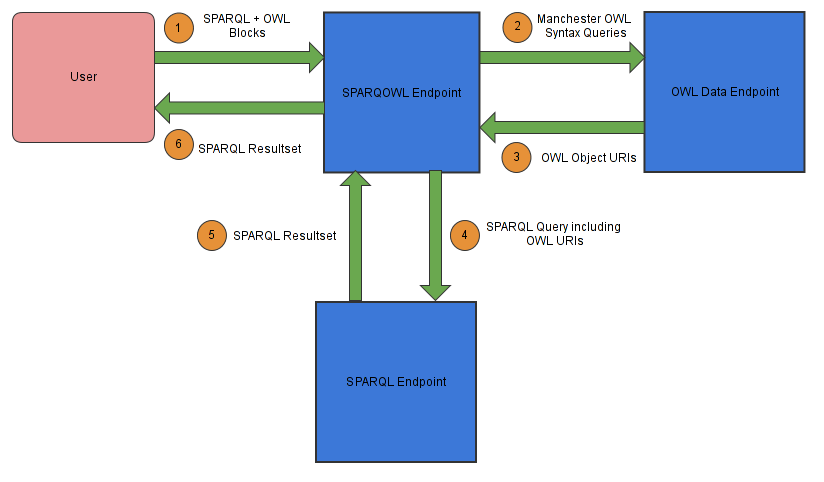
\includegraphics[width=\textwidth]{sparqowl.png}
  \caption{Basic Workflow of a SPARQOWL Request}
  \label{fig:sparqowl_request}
\end{figure}

A number of tools were used during the development process to ease navigation,
research and debugging:

\begin{description}
    \item[vim] This text editor provides advanced features such as macros and
    quick code navigation and debugging.
    \item[Netbeans] This IDE was used for the Java development aspects of the
    problem due to its advanced navigation, documentation and build tools.
    \item[git] Git was used for all aspects of the project for version control.
    New approaches were first prototyped in a new branch and successes were
    merged back into the master development branch.
\end{description}

\subsection{OWL Endpoint}

\subsubsection{Design}

The OWL endpoint will be a simple HTTP REST-like API which wraps code around an
OWL reasoner. The software will load a set of ontologies which any queries given
to the server will be run against, run the reasoner against them, and then set
up a simple server to accept Manchester OWL Syntax requests and return the
results in a machine-readable format.

The software uses the object orientated paradigm (as is natural for Java), along
with the observer pattern for the HTTP server and several hash map data models
for storing and processing ontology data.

In \ref{fig:requestclass}, the class diagram for the component of the software
which handles ontology loading and requests against the ontology. The
RequestManager holds a number of QueryEngines, which each hold and handle class
queries for a loaded ontology.

\begin{figure}[h!]
  \centering
  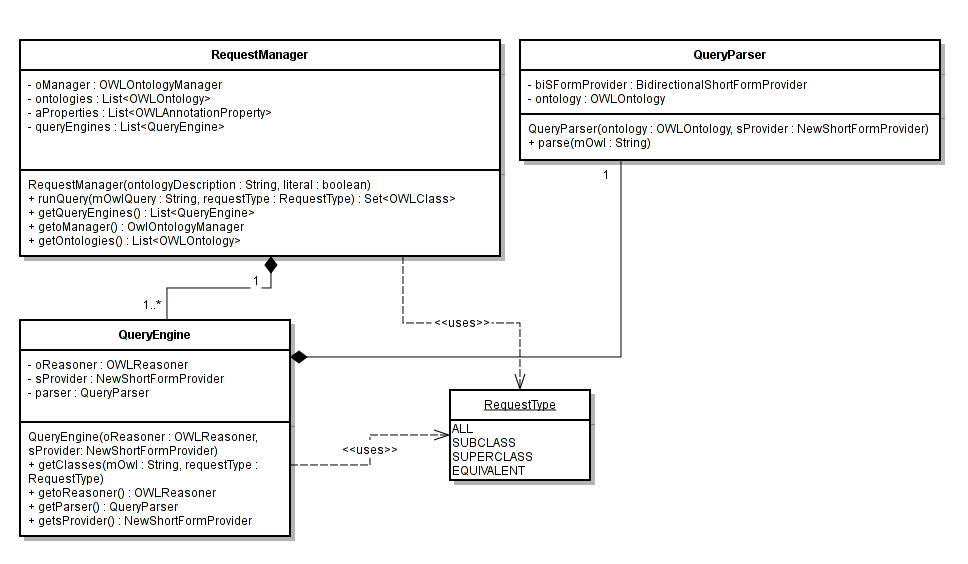
\includegraphics[width=\textwidth]{sparqowlapi.png}
  \caption{SPARQOWL API Request Class Diagram}
  \label{fig:requestclass}
\end{figure}

\subsubsection{Implementation}

Java was chosen to implement the OWL data endpoint, primarily to make use of the
extensive and ubiquitous OWLAPI library - which provides a number of useful
functionalities and features useful for this application, including helper
functions for parsing Manchester OWL Syntax, class expressions, ontology loading
and representation. Moreover, its support for several other pieces of software
(several types of reasoners, for example) means that the program remains
extensible and adaptable to new purposes.

The initial stages of the program startup are the following:

\begin{enumerate}
    \item Load specified ontologies into an ontology manager. 
    \item Perform reasoning on a set of ontologies and store the results.
    \item Generate a list of short-form labels for the classes in the
    ontologies.
    \item Create a set of query managers with the loaded ontologies to handle
    any future requests.
    \item Start a HTTP API listener with code to handle any queries.
\end{enumerate}

The list of ontologies are provided to the application as a list of
URIs in a text file. OWLAPI accepts most serialisation formats including OWL,
OBO and XML - so there aren't too many restrictions on the acceptable formats. 

Semantic reasoning is then performed on all of the loaded ontologies using the
ELK reasoner. The choice to use the ELK reasoner was made due to the fact it's
open source, is included by default in OWLAPI and supports the OWL 2 EL profile
- suitable for reasoning large biological ontologies at a reasonable speed. 
However, OWLAPI implements a standard interface for reasoner libraries and 
therefore any reasoner could potentially be used in the application.

To simplify querying, the ontologies' objects and classes are then iterated and
have their labels extracted. Labels are a 'human-friendly' name for a class -
e.g. 'adaxial cell' rather than 8951054, and this process allows the friendly
names to be used to query classes using the Manchester OWL Syntax. 

A custom short form provider (a subclass of the one included in OWLAPI) is then 
passed the annotations in order to create a bi-directional mapping between the
labels and the entities' (classes and instances) contained in the ontologies.
This allows for easy querying using the short-form label for OWL classes. It is
necessary to use a customised short form provider because while the Manchester
OWL Syntax uses single quotes to identify class labels which are formed of
multiple words, the default short form provider does not create mappings which
surround annotations with single quotes - making it impossible to query them
from such a parametised variable in a Manchester Owl Syntax expression.

Each ontology is loaded into its own QueryEngine class, which provides
functionality for retrieving a set of relevant classes from its ontology given a
valid class expression - then returning them in a HashMap.

Once this is done, the HTTP server will be started - exposing the simple API. 
The workflow of a request made to the server will be as follows:

\begin{enumerate}
    \item Retrieve Manchester OWL Syntax query.
    \item Convert the Manchester OWL Syntax query to a class expression (able to
    be queried against an ontology).
    \item Retrieve relevant objects from the ontologies.
    \item Serialise these objects in a machine-readable format and return them 
    to the collector.
\end{enumerate}

Jetty is used to create the HTTP server, since it is a simple HTTP server
library available for Java - implementing the required functionality without any
bloat, using in-built Java classes and thereby working towards the goal of
keeping the codebase light and extensible. The server uses an
observer-observable patter, and a single class instantiates the server while a
custom handler is attached to handle any requests. This is a common pattern used
for HTTP APIs, and allows for easy extensions for handling further parameters
and routes to the application.

A request sent to the server is a simple GET request including the Manchester
OWL Syntax format (with characters unacceptable in URIs parsed into HTML
entities and then converted back by the server - a single quote is converted to
\%20, for example), an example may be:

\begin{lstlisting}
http://jagannath.pdn.cam.ac.uk:9090/?query=has\_part\%20some\%20\%27plasma\%20membrane\%27
\end{lstlisting}

The listener sanitises the input and converts HTML entities back into their real
characters. It then sends the Manchester OWL Syntax request to the
RequestManager, along with any other relevant parameters which were passed with
the query. If the request was malformed, or did not include a query, an error
will be returned encoded in a JSON document. 

The RequestManager, containing the set of QueryEngines with the loaded
ontologies, then uses the QueryParser class to convert the Manchester OWL Syntax 
query to a class expression, utilising a number of in-built OWLAPI queries to do
so. A class expression is a generalised and standardised machine-readable OWL
class format usable with other OWLAPI functions (without the need for individual
conversion). The most common error encountered in such a request is a malformed
Manchester OWL Syntax query, and in such a case the parser will return an error
stating the nature of the error; when this happens, it is caught and an error
message is sent back to the originator of the request with the error message
encoded in JSON.

The RequestManager then iterates the QueryEngines and thereby the
ontologies, asking each for a set of relevant classes to the class expression
passed as a parameter - then collating the accrued HashMaps into a single
HashMap.

The QueryManager finds relevant classes to the given class expression by
collating equivalent classes, subclasses and superclasses (in terms of the class
hierarchy). It also has the potential to return instances, though this
functionality is not enabled in the prototype, since this is generally not
useful for biological ontologies - which generally represent a structure such as
an animal model, rather than an instance of a particular animal.

Since these various classes are relevant in different types of use case, there
is also a \emph{type} parameter available in the query - either \emph{subclass},
\emph{equivalent}, \emph{superclass} or \emph{all}, which will return only its
respective type of match from the given ontologies. If the parameter is omitted,
then all types of match will be returned. If no relevant classes are found, an
empty set will be returned.

Following this, it has a full list of relevant classes to the original query,
which it then uses the GSON library\cite{gson} (a Google-produced JSON library) to convert 
the classes into JSON format. The JSON is then returned to the Jetty
RequestHandler, which returns the data to the requestee.

\subsubsection{Testing and Documentation}

Testing is undertaken in this application by a number of unit tests. Basic
sanity tests such as checking the integrity of loaded data from an ontology are
used alongside tests which query the server and expect a particular response.
The tests use an example Pizza ontology found on the web, which is commonly
used for teaching and tutorials on the subject of OWL ontologies and querying.

The program itself includes a full set of JavaDoc which describes the public and
private methods included, designed to give an overview of the workflow of the
program and flow involved. A README file included in the distribution of the
program also describes basic information on how to run the program, as well as
information about configuration, such as populating the file from which to load
the ontologies. This document also provides an overview of the underlying design
and decisions taken during the development of the program. 

\subsection{SPARQL Extension}

The SPARQL extension takes place in the form of a wrapper around a script which
sends a SPARQL query, first evaluating the script for any OWL blocks - in the
case of which it sends an OWL query to the endpoint and includes any resulting
classes in the query in place of the OWL block.

The script is largely procedural, making use of functions for the processing of
the query and OWL data. This approach was chosen over object orientation due to
the simplicity of the script.

\subsubsection{SPARQL Syntax}

As described in the State of The Art, there is already a SERVICE keyword
included in the SPARQL language which provides a good model for sending a text
query to a remote endpoint, in terms of the syntax.\cite{sservice} 

\begin{lstlisting}
SERVICE <http://nourishedcloud.com/turtles> { 
    ?s tu:name ?name . ?s tu:owner ?owner
}
\end{lstlisting}

Evidenced above, the SERVICE block includes a URI which indicates a remote
SPARQL endpoint, then includes a SPARQL query to send the server - upon
execution and return of the results they are included in the resultset of the
rest of the query.

For an OWL query the pattern will be very similar - we want to send a Manchester
OWL Syntax Query to a remote OWL endpoint, and combine the resulting classes
with the resultset. Therefore, my software includes an 'OWL' block to the SPARQL 
language, which uses a similar syntactic pattern to the SERVICE keyword:

\begin{lstlisting}
OWL SILENT EQUIVALENT <http://realispicio.us:9090> {
    has_part some 'plasma membrane'
}
\end{lstlisting}

There are four properties to the above query:

\begin{description}
    \item[OWL] The OWL keyword will designate the beginning of an OWL block
    denoting the beginning of the description for a query to be sent to a remote
    OWL endpoint.
    \item[SILENT] This is an optional keyword, which if included will mean that
    no results are integrated if a query fails but the query will continue,
    while if it isn't set and a query fails the SPARQL query will be halted and
    return an error message.
    \item[EQUIVALENT] This flag may contain either \emph{EQUIVALENT},
    \emph{SUPER} or \emph{SUB}, which indicates to the remote OWL endpoint
    which type of class relevant to the following class description is required.
    If ommitted, all are returned.
    \item[IRI] The IRI, contained between angled brackets following the OWL
    keyword, will define the URI of the remote OWL endpoint.
    \item[Query] Following, between the curly brackets, will be a Manchester OWL
    Syntax query referring to relevant objects to be returned to the query.
\end{description}

Upon parsing the OWL block the syntax will send a query to an OWL reasoner
endpoint, and integrate the returned results into the query. 

\subsubsection{Syntax Implementation}

To preserve a simple proof-of-concept and prototype implementation of the
software, as well as retaining flexibility in the case of changing project
parameters, we approached this project with a simple solution in the form of a
PHP script. PHP also chosen because of its relative flexibility (acceptance of
input from both the command line and the Web), along with the existence of a
well-supported SPARQL library.

\begin{enumerate}
    \item Input the SPARQL query into the script.
    \item Scan the script for OWL blocks (syntax described above).
    \item Run any OWL queries.
    \item Replace the OWL block with the resultset from the OWL query.
    \item Run the SPARQL query.
    \item Return the full resultset.
\end{enumerate}

In terms of inputting the SPARQL query into the processing script, it supports
being run both from the command line and over the web, by checking whether it
was invoked from a web server or from the command line - then pulling the input
data from the appropriate source (either from the web form in POST data, or command
line arguments specifying either a file or a plain text query).

Before handling the SPARQL query, a simple regular expression is used to find
all occurences of the OWL block syntax described above. It then iterates through
these occurences, and uses the data extracted from them by the regular
expression to send the given Manchester OWL Syntax Query to the specified OWL
Endpoint.

The endpoint returns appropriate classes given the OWL query in JSON format, or an 
error. In the case of valid classes being returned, the JSON will be parsed for
the IRI and class names of said classes, then replacing the OWL block in
the query itself with the data about the returned classes inline in the query.
This would look like the following when querying relevant classes to the adaxial
cell in the Zebrafish ontology\cite{zfin}:

If the optional \emph{SILENT} keyword was used in conjunction with the OWL block
in question, and there was an error receiving any data from the remote OWL
enpoint, then the OWL block is simply deleted and the program continues either
processing and remaining OWL blocks, or will continue to execute the SPARQL
query. Otherwise, the program will exit and return an error message to the user stating
the the OWL request failed - including an error message returned from the OWL endpoint.

\begin{lstlisting}
VALUES (?iri ?id) { 
    ( http://purl.obolibrary.org/obo/#ZFA\_0009000  ZFA\_0009000 ) 
    ( http://www.w3.org/2002/07/owl#Nothing  Nothing )
}
\end{lstlisting}

Once all of the OWL blocks have been traversed and evaluated without error, the
SPARQL query will be made to a given remote endpoint. To perform this, the 
PHP-SPARQL-Lib library\cite{phpsparqllib} is used, which provides a class to 
construct, query and handle result sets from remote SPARQL endpoints using CURL.

Once the SPARQL query has been completed, the results will be displayed to the
user in an appropriate manner - either on a web page or printed to the executing
terminal.

As an example, a simple SPARQL query including an OWL block like so, which asks
for classes in the biology ontology//TODO CITE for classes which have a 'plasma
membrane' as a part:

\begin{lstlisting}
SELECT * WHERE {}
OWL <http://jagannath.pdn.cam.ac.uk:9090> {
    has\_part some 'plasma membrane'
}
\end{lstlisting}

The OWL block would first be identified, and then the given Manchester OWL
Syntax query would be sent to the specified endpoint and the block itself would
then be replaced by a list of the resulting values before being executed against
a SPARQL endpoint:

\begin{lstlisting}
SELECT * WHERE {} 
VALUES (?iri ?id) { 
    ( http://www.w3.org/2002/07/owl##Thing Thing ) 
    ( http://purl.obolibrary.org/obo/#GO\_0030313 GO\_0030313 ) 
    ( http://purl.obolibrary.org/obo/#GO\_0012505 GO\_0012505 ) 
}
\end{lstlisting}

The limitations of this addition in terms of actually using the returned class
URIs for matching against RDF datastores is that there is often a mismatch
between the URI prefixes and ID formats between OWL ontology class IDs and the
IDs which class annotations in RDF datasets use.

For exmaple, the biomodel ontology's RDF datastores use the following IRI to annotate a
acetylcholine-gated channel complex:

\begin{lstlisting}
http://identifiers.org/go/GO:0005892
\end{lstlisting}

Meanwhile, the OWL Gene Ontology uses :

\begin{lstlisting}
http://purl.obolibrary.org/obo/GO\_0005892
\end{lstlisting}

Due to this, URIs returned by the OWL ontology won't actually be matched against
the models in the biomodel ontology.

This is a well known problem, and originates from legacy ontology development
whereby ontologies would simply use an id (e.g.) GO\_0005892 to identify a class.
However, RDF datastores use URIs as predicate values and therefore RDF
datastores would essentially 'make up' prefixes for for their annotations.

Since then, OBO decided on a standardised format for annotation URIs
(http://purl.obolibrary.org/obo/), but unfortunately RDF datastores have not yet
been updated to support this new format. 

Several approaches have been made to address this issue, such as
http://identifiers.org, which resolves and finds links between identifiers. But
in essence this means further ID formats have been created beyond those which
already exist! 

Thankfully, IRI and ID formats are relativley easy to tranform and then REPLACE
functionality of the SPARQL language, the following example for example takes
the URIs provided by the OWL endpoints and transforms then to a format
acceptable to the RDF datastore.

\begin{lstlisting}
BIND (IRI (REPLACE(STR(?id), "http://purl.obolibrary.org/obo/GO\_",
"http://identifiers.org/go/GO:")) as ?newgoid)
\end{lstlisting}

This does not compromise the usability of the sofware, however it adds an
extra level of complexity wich must fall on the creator of the SPARQL query to
create a workable theory.

Hopefully, in time the maintaners of the RDF datastores will work towards
uniformity in annotation IDs, simplifying the process of OWL integration using
this method.

\subsubsection{Web Interface}

The web interface is also a simple piece of software, it existing as a simple
HTML form which accepts a SPARQL (with potential OWL block) query along with a
remote endpoint to execute it against. Upon submitting the HTML form, the script
described in the previous section is passed POST data from the page, then
executing the query and printing the results to the screen, or displaying an
error message in the case of an error.

* Insert screenshot

\subsubsection{Testing and Documentation}

The SPARQL extension implementation's design is described by this document. The
script itself also includes ample commenting to help a reader understand the
flow and meaning of the code involved in the software.

In terms of user-end documentation, The web interface also includes a link to a 
basic page with a basic description
about the OWL block and how to use it - including examples. Furthermore, a
README is included with the distribution of the project which describes its
purpose as well as including information also found on the web interface's help
page.

\subsection{Use Cases and Examples}

The BioModels database is a large RDF datastore which stores models of
biological processes, its latest release included more than 140,000 models - all
of which are cited and supported by peer-reviewed scientific literature.

Models also include annotations under various properties, which are URIs which 
refer to classes in other ontologies (usually OWL) thereby linking that property
of the model with a class in another dataset. 

A common example is an annotation on isVersionOf, so the biomodel entry for a
\emph{biliganted basal state} is annotated to \emph{GO:0005892}, or the
\emph{acetylcholine-gated channel complex}.

Example 3 given on the SPARQL endpoint provided for the BioModels database
retrieves all models in the datastore which are annotations to the
acetylcholine-gated channel complex, with the following query (prefixes ommited):

\begin{lstlisting}
SELECT ?modelElement ?elementType ?qualifier WHERE { 
  ?modelElement ?qualifier <http://identifiers.org/go/GO:0005892> .  
  ?qualifier rdfs:subPropertyOf sbmlrdf:sbmlAnnotation . 
  ?modelElement rdf:type ?elementType 
}
\end{lstlisting}

The annotation must be referred to by its URI
(http://identifiers.org/go/GO:0005892), and therefore any user wishing to use a
similar or more complicated query must use a desktop ontology utility such as
Protege to find the relevant class, and then paste the necessary ID into the query. 
With the SPARQL OWL extension one can simply query this ID directly from an OWL
endpoint using its label and implant it into the query. So the equivalent would 
be (prefixes ommitted):

\begin{lstlisting}
SELECT ?newgoid ?modelElement ?elementType ?qualifier WHERE {
  OWL ?id EQUIVALENT <jagannath.pdn.cam.ac.uk:9090> { 'acetylcholine-gated channel complex' }
  BIND (IRI (REPLACE(STR(?id), "http://purl.obolibrary.org/obo/GO_", "http://identifiers.org/go/GO:")) as ?newgoid)

  ?modelElement ?qualifier ?newgoid .
  ?qualifier rdfs:subPropertyOf sbmlrdf:sbmlAnnotation .
  ?modelElement rdf:type ?elementType
}
\end{lstlisting}

Since the OWL data endpoint can be loaded with several ontologies at once, 
one can also query for annotations from several ontologies at once (for example
the protein sequence ontology).

Furthermore, since one can additionally query for superclasses and subclasses
(or both) of the given Manchester OWL Syntax class expression (and the datastore 
is queried for all results returned by the OWL block), a wider range of useful and
relevant results may be retrieved from the RDF datastore - since annotation IDs
are returned for all classes in the ontology relevant to the expression in the
given hierarchical direction.

Additionally, since any Manchester OWL Syntax class expression can be provided 
in the OWL block, more advanced queries can be made to retrieve annotations to
search against. For example, this query retrieves annotation IDs for all classes
which are a part of the plasma membrane in the gene ontology, when making a
remote query to the https://www.ebi.ac.uk/rdf/services/biomodels/sparql SPARQL
endpoint with the OWL block preprocessor (prefixes ommitted):

\begin{lstlisting}
SELECT ?newgoid ?modelElement ?elementType ?qualifier WHERE {
  OWL ?id SUPERCLASS <jagannath.pdn.cam.ac.uk:9090> { has\_part some 'plasma membrane' }
  BIND (IRI (REPLACE(STR(?id), "http://purl.obolibrary.org/obo/GO\_", "http://identifiers.org/go/GO:")) as ?newgoid)

  ?modelElement ?qualifier ?newgoid .
  ?qualifier rdfs:subPropertyOf sbmlrdf:sbmlAnnotation .
  ?modelElement rdf:type ?elementType
}
\end{lstlisting}

Or query for all items annotated as being part of apoptosis - processes involved
in cell death:

\begin{lstlisting}
SELECT ?newgoid ?modelElement ?elementType ?qualifier WHERE {
  OWL ?id SUBCLASS <jagannath.pdn.cam.ac.uk:9090> { part\_of some apoptosis }
  BIND (IRI (REPLACE(STR(?id), "http://purl.obolibrary.org/obo/GO\_", "http://identifiers.org/go/GO:")) as ?newgoid)

  ?modelElement ?qualifier ?newgoid .
  ?qualifier rdfs:subPropertyOf sbmlrdf:sbmlAnnotation .
  ?modelElement rdf:type ?elementType
}
\end{lstlisting}

As previously mentioned many RDF datastores include outdated annotation IDs, in
this case using a different URI and prefix seperation character. In these
examples this is rectified by using the REPLACE functionality of the SPARQL
language to modify the returned IDs to conform to the required format. For an
unknown reason this actually slows the query down somewhat, though in future the
annotation IDs used in RDF datastores will be updated to conform to their
definitions in the ontologies.

An OWL endpoint can currently be found running at
\emph{http://jagannath.pdn.cam.ac.uk:9090/}, loaded with several ontologies -
particularly the Gene Ontology.

Additionally, an instance of the SPARQOWL web interface can be found at
\emph{http://jagannath.pdn.cam.ac.uk/sparqowl/}.

\section{Conclusion}

\subsection{Evaluation}

Through the research and execution of this project, it was found that there was
indeed no current method by which to use a human-writable syntax to directy query OWL
ontologies on the web, useful particularly for querying models in RDF datastores
annotated with IDs from OWL ontologies.

It was found that SPARQL includes provisions for manipulating OWL ontologies by
first converting them to an RDF format, however this sacrificed several endemic
features of the OWL technology - including semantic reasoning and expressive
power.

Several approaches were attempted, and eventually these issues were solved by
creating two pieces of software. One, an extension to the SPARQL language which
allows a user to provide an OWL class description using the compact and human
readable format and a remote URI, allows a user to return reasoned classes
relevant to the given expression.

The second was an 'OWL Endpoint,' supporting the OWL block functionality, allows
the user to obtain classes from a number of configurable ontologies given a
class description providied in a Manchester OWL Syntax string. This solution is
useful both for the aforementioned SPARQL extension, but also for any potential
application which requires the remote querying of OWL classes over the web.

\subsection{Summary of Contributions}

Implemented a demonstration of an extension to the SPARQL language to allow
remote querying of a set of OWL ontologies at
a given data endpoint using Manchester OWL Syntax. Relevant results are then
included in the OWL resultset and can
interact with the rest of the query as a regular 'list' of data. The script can
either be used from the command line or
through the web.

Implemented a basic Web front-end for making SPARQL queries, designed to make
available the previously noted implementation of
the OWL querying functionality on the Web.

Created a simple REST Web API to constitute an OWL data endpoint for ontology
querying, with a similar pattern to SPARQL
endpoints. It allows a user to make a Manchester OWL Syntax query, describing a
set of relevant classes, which are then
matched against a number of in-built and reasoned ontologies, then returned in
JSON format.

\subsection{Future Work}

\subsubsection{Re-implement current SPARQL functionality in other languages}

To increase the universal availability of this functionality, it would be a good
idea to implement it in other languages which
have a SPARQL library. The design pattern for the base OWL block functionality
is rather simple so it would be easy to port
to other languages either by myself or someone who needs it for a specific
purpose with a specific set of technologies. PHP
was chosen initially since the focus was on Web availability, and most web-based
SPARQL endpoints which humans interact with
are using PHP. However, there exist similar libraries for languages such as
NodeJS, Python, C and others.

\subsubsection{Provide Integrated SPARQOWL Endpoint}

Another approach which could be taken to make this functionality more available
is to create an instance of a SPARQL endpoint which actually includes support
for the OWL block - or perhaps integrate it into the OWL endpoint itself. This
presents several problems however, as current SPARQL endpoints generallu do not
support federated queries themselves, and are usually loaded with their own
datasets. Generic SPARQL endpoints are generally rather uncommon for security
reasons - either the case of malformed and malicious datasets, or resource
overuse.

\subsubsection{Extend actual SPARQL Syntax}

In researching the implementation of the OWL block addition to SPARQL, the
initial thoughts were to perform this by actually extending the language itself.
To do this, the only seemingly viable option was to extend Apache Jena, which is
a major and widely used semantic web framework written in Java which includes the 
ARQL SPARQL compiler. 

The original plan was to build the extra syntax into ARQL in Jena, and
distribute a modified version of the software while requesting the changes be
merged with the main codebase.

However, after further investigation this approach was deemed unsuitable because
of the perceived inextensibility of the ARQL codebase, which makes use of a
large amount of magic numbers and goes largely undocumented. [am I allowed to
say this?]

Eventually, it would be a superior solution to actually extend the SPARQL
language itself - both by extension of the SPARQL
specification and through an extension in the reference implementation of SPARQL
(ARQ); this would increase visibility of the
project, as well as working towards the new features being more widely
supported.

\subsubsection{Combination with SERVICE}

As previously mentioned, there is already a SERVICE keyword included in the
SPARQL language, which follows the model of sending a HTTP query to a remote
endpoint and integrating the results with the local resultset.\cite{sservice}

Currently, it only supports remote SPARQL endpoints, and it was decided not to 
extend this construct to include support for an OWL endpoint during the course
of theis project, as this would mean any resulting implementation would break 
the terms of the SPARQL specification. However, it may be suggested to the W3C 
in future to combine these constructs as a matter of syntactic efficiency. 

The pattern between the SERVICE and OWL keywords are very
similar. Because of this, the extension of the SERVICE keyword to include OWL
endpoints should not be too difficult, and carries the additional benefit of
providing a reasonable and extendable framework for the further extension of the
keyword to include and support other such simple endpoints which may be
developed in the future (supporting further data integration with a standard
interface).

\subsubsection{Data Integration From Other Sources}

While connecting OWL and RDF datastores in this manner already allows for a lot
of new work to be done, there are other semantic data formats which currently do 
not support easy data integration. I think that SPARQL serves as a good base for 
any further data integration, given its wide adoption and currently existing 
support for many different types of data. Examples of ontology formats which
could be integrated are CASL, CycL, DOGMA and KIF.

Such additions could potentially save a lot of work which takes place in
manually creating mappings between existing ontologies and technologies which
are designed for intercommunication; for example, mappings between RDF/OWL ontologies and the
SNOMED medical vocabularies\cite{snomed1}. In a world of data integration which does not
compromise the endemic features of a particular technology, such a choice would
not impact the global federation, integration and intercommunication between
different sources for practical uses.

\subsubsection{More Functionality in the OWL API}

The current implementation of the OWL API endpoint is very simple, designed as
what is mainly a proof of concept. As mentioned in the design
section, the API currently searches objects over a set of default ontologies
found at the\cite{obofoundry}. While this provides a useful set of
ontologies for queries, it is somewhat inflexible. Currently, if a user wishes
to query an ontology which isn't included in the endpoint, they
would have to download a copy of the software and modify the list of ontologies
- then running it themselves.

To remedy this, I would plan on keeping the current functionality in terms of a
default set of ontologies, but implement an additional query
parameter which allows the user to list a set of URIs pointing at ontologies to
reason and query. While this would be a useful feature, it
presents several design challenges: 

\begin{itemize}
    \item Care would have to be taken to prevent damage to the server by being
    passed an ontology either maliciously formed or too large for the server to
    reasonably process.
    \item Additions would have to be made to the OWL block syntax in the SPARQL
    extension to specify a set of ontologies to reason over.
    \item Ontology loading and reasoning would have to take place upon the
    request being executed, which could potentially be rather slow depending on
    the size and amount of ontologies.
\end{itemize}

Whilst going forward with this project, it may also be worth drafting a formal
specification for what constitutes an 'OWL endpoint,' similar
to that which exists for SPARQL endpoints. This would be useful for an
authoritative source on functionality, as well as being able
to dictate necessary functionality for any further and alternative
implementations. However, due to what is rather an implementation monopoly on
OWL manipulation which lies with OWLAPI, it is unlikely that such functionality
could be easily replicated using another library.

Further configuratbility in the application would also be useful, from basic
configuration such as the address and port to which the server binds, to which
reasoner the application should use. This would be useful for allowing the
application to support a wider range of uses without expecting users to have to
modify it. This could be implemented either with command line arguments or
creating a configuration file which contains such directives.

There is also a bug whereby OWLAPI refuses to reason over ontologies loaded from
the IMPORT closure of parent OWL ontologies - while also refusing to explicitly
load then once having done so. This makes it rather difficult to load a large
amount of ontologies at once due to clashing. This could be solved by either
somehow forcing OWLAPI to reason with and retrieve classes from these
ontologies, or perhaps by dynamically ignoring the importation of further
ontologies from import closures.

Similar to SPARQL endpoints, which are often accompanied by web-frontends, it
may be a good idea to develop a web-frontend which supports only Manchester OWL
Syntax querying. This would assist in the goal of reaching feature parity in
querying OWL ontologies.

Further functionality could also be added in future to utilise more features of
OWLAPI, such as the modification of ontologies. With these features, it could
become more useful to front-end applications with write capabilities. This would
probably require the implementation of authentication (using basic HTTP
authentication or OAuth, for example) and further security features such as rate-limiting.

\subsubsection{Possibly Extend OWLLink API}

Despite not supporting Manchester OWL Syntax queries, OWLLink API is a large and
developed project. For this reason, it may be worth doing some
more work into researching whether the implemtation of Manchester OWL Syntax
queries is faesible.

\begin{thebibliography}{9}

\bibitem{semweb}
  Tim Berners-Lee et al,
  \emph{The Semantic Web}.
  Feature Article, Scientific American
  May 2001.

\bibitem{rdfprimer}
 Tim Berners-Lee et al,
 \emph{RDF Primer}.
 W3C,
 2004.

\bibitem{jena}
  McBride, Brian.
  "Jena: A semantic web toolkit." 
  IEEE Internet computing 6.6
  (2002): 55-59.

\bibitem{sparql}
  Eric Prud'hommeaux, Andy Seaborne,
  \emph{SPARQL Query Language for RDF}.
  W3C,
  January 2008.

\bibitem{fact}
  Tsarkov, Dmitry, and Ian Horrocks. "FaCT++ description logic reasoner: System description." Automated reasoning. Springer Berlin Heidelberg, 2006. 292-297.

\bibitem{sparqlquerying}
  Quilitz, Bastian, and Ulf Leser. 
  "Querying distributed RDF data sources with SPARQL." 
  The Semantic Web: Research and Applications. 
  Springer Berlin Heidelberg, 
  2008. 524-538.

\bibitem{pharmgkb}
  Allison, M., NCATS launches drug repurposing program.
  Nat Biotechnol,
  2012: 30(7): p. 571-2.
  
\bibitem{drugrepurposeinitial}
  Hoehndorf, R., A. Oellrich, D. Rebholz-Schuhmann, P.N. Schofield, and G.V. Gkoutos,
  Linking PharmGKB to phenotype studies and animal models of disease for drug repurposing. 
  Pacific Symposium on Biocomputing (PSB), 
  2012: p. 388-399.

\bibitem{sparqlandowl}
  Kollia, Ilianna, Birte Glimm, and Ian Horrocks. "SPARQL query answering over
  OWL ontologies." The Semantic Web: Research and Applications. Springer Berlin
  Heidelberg, 2011. 382-396.

\bibitem{zfin}
  Sprague, J., L. Bayraktaroglu, Y. Bradford, T. Conlin, N. Dunn, D. Fashena, K. Frazer, M. Haendel, D.G. Howe, J. Knight, P. Mani, S.A. Moxon, C. Pich, S. Ramachandran, K. Schaper, E. Segerdell, X. Shao, A. Singer, P. Song, B. Sprunger, C.E. Van Slyke, and M. Westerfield, 
  The Zebrafish Information Network: the zebrafish model organism database provides expanded support for genotypes and phenotypes. 
  Nucleic. Acids Research,
  2007: p. gkm956+.

\bibitem{wormbase}
  Harris, T.W., I. Antoshechkin, T. Bieri, D. Blasiar, J. Chan, W.J. Chen, N. De La Cruz, P. Davis, M. Duesbury, R. Fang, J. Fernandes, M. Han, R. Kishore, R. Lee, H.-M. M\"uller, C. Nakamura, P. Ozersky, A. Petcherski, A. Rangarajan, A. Rogers, G. Schindelman, E.M. Schwarz, M.A. Tuli, K. Van Auken, D. Wang, X. Wang, G. Williams, K. Yook, R. Durbin, L.D. Stein, J. Spieth, and P.W. Sternberg, 
  WormBase: a comprehensive resource for nematode research,
  Nucleic Acids Research,
  2010. 38(suppl 1): p. D463-D467.

\bibitem{ddp}
  Ullrich Hustadt, Boris Motik, Ulrike Sattler,
  Reducing SHIQ Description Logic to Disjunctive Datalog Programs,
  KR,
  2004.

\bibitem{owl2xml}
  Motik, Boris, Bijan Parsia, and Peter F. Patel-Schneider. "OWL 2 web ontology
  language XML serialization." W3C Recommendation, W3C–World Wide Web Consortium
  (2009).

\bibitem{flybase}
  Drysdale, R. and FlyBase Consortium, FlyBase : a database for the Drosophila research community.
  Methods in molecular biology (Clifton, N.J.), 2008. 420: p. 45-59.

\bibitem{desclogic}
 Franz Baader, Deborah L. McGuinness, Daniele Nardi, Peter F. Patel-Schneider,
 \emph{The Description Logic Handbook - Theory, Implementation and Actions}.
 Cambridge University Press,
 March 2003.

\bibitem{owlprimer}
  Pascal Hitzler et al,
  \emph{OWL 2 Web Ontology Language Primer (Second Edition)}.
  W3C,
  December 2012.

\bibitem{owlprofiles}
  http://www.w3.org/TR/owl2-profiles/
  W3C,
  Accessed: 27/04/2014.

\bibitem{humontology}
  Nicole L. Washington et al,
  Linking Human Diseases to Animal Models Using Ontology-Based Phenotype Annotation,
  Plos Biology,
  November 2009.

\bibitem{pato}
  Gkoutos, G.V., E.C. Green, A.-M.M. Mallon, J.M. Hancock, and D. Davidson,
  Using ontologies to describe mouse phenotypes. 
  Genome biology, 
  2005.

\bibitem{gson}
  Google Inc.
  https://code.google.com/p/google-gson/
  Accessed: 20/02/2014

\bibitem{semwebdiscovery}
  D.J. Wild, et al.,
  Systems chemical biology and the Semantic Web: what they mean for the future of drug discovery research,
  Drug Discov Today,
  2012.

\bibitem{tableau}
  M. Schmidt-Schauß and G. Smolka. 
  Attributive concept descriptions with complements.
  Artificial Intelligence, 48(1):1–26, 1991.

\bibitem{phpsparqllib}
  Christopher Gutteridge \& University of Southampton,
  PHP-SPARQL-Lib,
  https://github.com/cgutteridge/PHP-SPARQL-Lib,
  Accessed 23/2/2014.

\bibitem{shoe}
  Luke, S., Spector, L, and Rager, D. 
  Ontology-Based Knowledge Discovery on the World-Wide Web. 
  Workshop on Internet-Based Information Systems at the 13th National Conference on Artificial Intelligence. 
  1996.

\bibitem{revisited}
  Shadbolt, Nigel, Wendy Hall, and Tim Berners-Lee. "The semantic web
  revisited." Intelligent Systems, IEEE 21.3 (2006): 96-101.

\bibitem{obofoundry}
  Obo Foundry
  http://obofoundry.org/
  Retrieved 17/04/2014.

\bibitem{syntweb}
  Robie, Jonathan, et al. 
  "The syntactic Web: Syntax and semantics on the Web."
  Markup Languages: Theory and Practice 3.4 
  (2001): 411-440.

\bibitem{phenoscape}
  Dahdul, W.M., J.P. Balhoff, J. Engeman, T. Grande, E.J. Hilton, C. Kothari, H. Lapp, J.G. Lundberg, P.E. Midford, T.J. Vision, M. Westerfield, and P.M. Mabee, 
  Evolutionary characters, phenotypes and ontologies: curating data from the systematic biology literature,
  PLoS One,
  2010. 5(5): p. e10708.

\bibitem{vph}
  de Bono, B., R. Hoehndorf, S. Wimalaratne, G.V. Gkoutos, and P. Grenon, 
  The RICORDO approach to semantic interoperability for biomedical data and models: strategy, standards
and solutions, 
  BMC Research Notes, 
  2011. 4(1): p. 313.

\bibitem{impc}
  Brown, S.D. and M.W. Moore,
  Towards an encyclopaedia of mammalian gene function: the International Mouse Phenotyping Consortium. 
  Dis Model Mech, 
  2012. 5(3): p. 289-92.

\bibitem{dbpedia-uses}
  DBPedia Use Cases,
  http://wiki.dbpedia.org/UseCases
  Retrieved 07/04/2014

\bibitem{reasonercompare}
  Kathrin Dentler, et al.
  Comparison of Reasoners for large Ontologies in the OWL 2 EL Profile,
  2010.

\bibitem{reasonerbenchmark}
  Juergen Bock, et al,
  Benchmarking OWL Reasoners,
  Workshop on Advancing Reasoning on the Web: Scalability and Commonsense,
  2008.

\bibitem{elplusplus}
  Franz Baader, Sebastian Brandt, Carsten Lutz,
  Pushing the EL Envelope,
  IJCAI'05 Proceedings of the 19th international joint conference on Artificial intelligence
  2005. p. 364-369.

\bibitem{dbpedia}
  Auer, Sören, et al. "Dbpedia: A nucleus for a web of open data." The semantic
  web. Springer Berlin Heidelberg, 2007. 722-735.

\bibitem{dbpediastats}
  Bizer, Christian, et al. "DBpedia-A crystallization point for the Web of
  Data." Web Semantics: Science, Services and Agents on the World Wide Web 7.3
  (2009): 154-165.

\bibitem{damloil}
  Horrocks, Ian. 
  "DAML+OIL: a Description Logic for the Semantic Web." 
  IEEE Data Eng. Bull. 25.1 
  (2002): 4-9.

\bibitem{daml}
  Coalition, DAML-S., et al. 
  "DAML-S: Web service description for the semantic Web." 
  The Semantic Web-ISWC. 2002.

\bibitem{oil}
  Fensel, Dieter, et al. 
  "OIL: An ontology infrastructure for the semantic web."
  Intelligent Systems, IEEE 16.2 
  (2001): 38-45.

\bibitem{psurveyor}
  Hines, Lisa E., Daniel C. Malone, and John E. Murphy. "Recommendations for
  Generating, Evaluating, and Implementing Drug‐Drug Interaction Evidence."
  Pharmacotherapy: The Journal of Human Pharmacology and Drug Therapy 32.4
  (2012): 304-313.

\bibitem{sesame}
Broekstra, Jeen, Arjohn Kampman, and Frank Van Harmelen. "Sesame: A generic
architecture for storing and querying rdf and rdf schema." The Semantic Web—ISWC
2002. Springer Berlin Heidelberg, 2002. 54-68.

\bibitem{rdfs}
  Brickley, Dan, and Ramanathan V. Guha. 
  "RDF vocabulary description language 1.0: RDF schema." 
  (2004).

\bibitem{snomed1}
  Hyvönen, Eero, et al. "Building a national semantic web ontology and ontology
  service infrastructure–the FinnONTO approach." The Semantic Web: Research and
  Applications. Springer Berlin Heidelberg, 2008. 95-109.

\bibitem{snomed2}
  Schulz, Stefan, et al. "The Semantics of Procedures and Diseases in SNOMED®
  CT." Methods of Information in Medicine 45.4 (2006): 354.

\bibitem{rdf}
  Klyne, Graham, and Jeremy J. Carroll. 
  "Resource description framework (RDF): Concepts and abstract syntax." 
  (2006).

\bibitem{ontology}
  Smith, Barry. 
  "Ontology." 
  The Blackwell guide to the philosophy of computing and information 
  (2003): 153-166.

\bibitem{jenardf}
  McBride, Brian. 
  "Jena: Implementing the RDF Model and Syntax Specification."
  SemWeb. 
  2001.

\bibitem{linkdata}
  Heath, Tom, and Christian Bizer. 
  "Linked data: Evolving the web into a global data space." 
  Synthesis lectures on the semantic web: theory and technology 1.1
  (2011): 1-136.

\bibitem{arq}
  Jena, Joseki, and Pellet Fuseki. 
  "Semantic web frameworks." 
  (2004).

\bibitem{pellet}
  Sirin, Evren, et al. "Pellet: A practical owl-dl reasoner." Web Semantics:
  science, services and agents on the World Wide Web 5.2 (2007): 51-53.

\bibitem{elk}
  Kazakov, Yevgeny, Markus Krötzsch, and František Simančík. "ELK: a reasoner
  for OWL EL ontologies." System Description (2012).

\bibitem{owlim}
  Kiryakov, Atanas, Damyan Ognyanov, and Dimitar Manov. "OWLIM–a pragmatic
  semantic repository for OWL." Web Information Systems Engineering–WISE 2005
  Workshops. Springer Berlin Heidelberg, 2005.

\bibitem{racerpro}
  Haarslev, Volker, et al. "The RacerPro knowledge representation and reasoning
  system." Semantic Web 3.3 (2012): 267-277.

\bibitem{hermit}
  Shearer, Rob, Boris Motik, and Ian Horrocks. "HermiT: A Highly-Efficient OWL
  Reasoner." OWLED. Vol. 432. 2008.

\bibitem{xml}
  Bray, Tim, et al. 
  "Extensible markup language (XML)." 
  World Wide Web Consortium Recommendation REC-xml-19980210. 
  http://www. w3. org/TR/1998/REC-xml-19980210
  (1998).

\bibitem{rest}
  Rodriguez, Alex. 
  "Restful web services: The basics." 
  Online article in IBM DeveloperWorks Technical Library 36 (2008).

\bibitem{uptake}
  Heath, Tom, John Domingue, and Paul Shabajee.
  "User interaction and uptake challenges to successfully deploying Semantic Web technologies." (2006).

\bibitem{sservice}
  Quilitz, Bastian, and Ulf Leser. 
  "Querying distributed RDF data sources with SPARQL." 
  The Semantic Web: Research and Applications. Springer Berlin Heidelberg, 
  2008. 524-538.

\bibitem{manchesterowl}
  Horridge, Matthew, et al. "The Manchester OWL Syntax." OWLed. Vol. 216. 2006.

\bibitem{bbcone}
  Raimond, Yves, et al. "Use of Semantic Web technologies on the BBC Web Sites."
  Linking Enterprise Data. Springer US, 2010. 263-283.

\bibitem{bbctwo}
  Kobilarov, Georgi, et al. "Media meets semantic web–how the bbc uses dbpedia
  and linked data to make connections." The semantic web: research and
  applications. Springer Berlin Heidelberg, 2009. 723-737.

\bibitem{kaon}
  Motik, Boris, and R. Studer. "KAON2–A scalable reasoning tool for the semantic
  web." Proceedings of the 2nd European Semantic Web Conference (ESWC’05),
  Heraklion, Greece. Vol. 17. 2005.

\bibitem{kaonabox}
  Motik, Boris, and Ulrike Sattler. "Practical DL Reasoning over large ABoxes
  with KAON2." (2006).

\bibitem{owllink}
  Liebig, Thorsten, et al. "OWLlink." Semantic Web 2.1 (2011): 23-32.

\bibitem{turtle}
  Beckett, David, and Tim Berners-Lee. "Turtle-terse RDF triple language." W3C
  Team Submission 14 (2008).

\bibitem{ntriples}
  Beckett, Dave, and Art Barstow. "N-Triples." W3C RDF Core WG Internal Working
  Draft (2001).

\bibitem{owllinkprotocol}
  Liebig, Thorsten, Marko Luther, and Olaf Noppens. "The OWLlink Protocol." OWLED.
2009.

\bibitem{prot}
Noy, Natalya F., et al. "Protege-2000: an open-source ontology-development and
knowledge-acquisition environment." AMIA Annu Symp Proc. Vol. 953. 2003.

\bibitem{protowl}
Knublauch, Holger, et al. "The Protégé OWL plugin: An open development
environment for semantic web applications." The Semantic Web–ISWC 2004. Springer
Berlin Heidelberg, 2004. 229-243.

\bibitem{shiq}
  Motik, Boris, Ulrike Sattler, and Rudi Studer. "Query answering for OWL-DL
  with rules." The Semantic Web–ISWC 2004. Springer Berlin Heidelberg, 2004.
  549-563.

Example OWLLink query:
http://owllink.org/owllink-httpxml-20091116/additional-examples/owllink-example-ClassQueries-request-20091116.xml

\end{thebibliography}

\end{document}
